\section{Results}

\subsection{Traits and diversification}

% NOTE: will need to update figure/panel refs if making no-delta models primary
% R: I am changing no delta as just D/P and prevous D/P as +delta

% E: I brutally shortened the text here and hence put all the models into one section for the "diversification" question.  But I think I retained all the ideas that were written out before.
% Much of what I removed was descriptions about which distributions are/aren't overlapping with one another.  I think that's easier for the reader to see in the figures than to read in the text.  But now the text says things like if some estimates are "different", so perhaps in Methods we should explain different = non-overlapping?
% For the former model comparison section, I moved the key conclusions into the paragraphs here and the mechanical details (bayes factor definition) into Methods.

Individual trait-dependent diversification inference, of ploidy and breeding system considered separately, each showed significant associations with net diversification differences. 
When considered together, however, the effect of breeding system dominated the effect of ploidy, although hidden factors played an important role as well.

When considering ploidy alone (D/P model), we found a greater net diversification rate for diploids than for polyploids, in agreement with \citep{mayrose_2011, mayrose_2015}.
This result holds with (\cref{figure:netdivall}A) or without (\cref{figure:netdivnodip}A) the diploidization parameter, though including diploidization shifts the net diversification rate of polyploids to be non-negative.
Incorporating a hidden state, however, removes the clear separation in diversification between diploids and polyploids (D/P+A/B model; \cref{figure:netdivall}B, \cref{figure:netdivnodip}B).
Thus, differences in net diversification are better explained by an unknown factor than by ploidy.
Statistical model comparisons show very strong support for including the hidden state and strong support for including diploidization (\cref{table:bayesfactors}).
% E: I removed the description of relative extinction results.  We don't discuss it for other models or show it in the main text, and I never really know what to make of that compound parameter.  But it's good that it's in the supp info.

When considering breeding system alone (I/C model, \cref{figure:netdivall}C), we found a larger net diversification rate for SI than for SC species, in agreement with \citet{goldberg_2010}. %B: moved \cref{} earlier; avoids seeming related to \citep{}
When a hidden state is included (I/C+A/B model), the large net diversification difference persists for one of the hidden states but is removed for the other (\cref{figure:netdivall}D).
Thus, differences in net diversification are best explained by both breeding system and an unknown factor, similar to results found by \citet{freyman_2018}.
% The transition rate from SI to SC is $q_{IC}=0.3$ for both the I/C and the I/C+A/B models.
The statistical model comparison shows very strong support for including the hidden state (\cref{table:bayesfactors}).

When considering ploidy and breeding system together (ID/CD/CP model), the net diversification rate for SI diploids was greater than for either SC diploids or SC polyploids, with or without diploidization (\cref{figure:netdivall}E, \cref{figure:netdivnodip}C).
It thus appears that the difference in net diversification with breeding system persists when ploidy is included in the model, but not the reverse.
The association of ploidy with net diversification in the D/P model (\cref{figure:netdivall}A, \cref{figure:netdivnodip}A) appears to be driven by the subset of diploids that are SI; among SC species, net diversification rates for diploids and polyploids are similar.
%
When a hidden state is included (IC/CD/CP+A/B model), the same general pattern remains when diploidization is prevented (\cref{figure:netdivnodip}D), although the higher net diversification rate of ID is less clear within one of the hidden states.
With diploidization, the net diversification rate of ID is still greater than CD within each hidden state, but diversification for P is highly uncertain and perhaps bimodal.
Statistical model comparisons show very strong support for including the hidden state and at most positive support for including diploidization (\cref{table:bayesfactors}).

\subsection{Pathways to polyploidy}

Evolution from self-incompatible diploids to self-compatible polyploids can proceed through two different pathways.
Determining the relative contribution of these pathways based on our estimated transition rates from the ID/CD/CP model, we find that the one-step pathway is more likely on short timescales and the two-step pathway is more likely on long timescales (\cref{figure:pathways}, left panels).
When not much time has elapsed, the one-step pathway is more likely because only one event need happen.
When more time has elapsed, the two-step pathway is more likely because the rate of loss of SI within diploids, $q_{IC}$, is greater than the rate of polyploidization for SI species, $\rho_I$ (\cref{suppfigure:IDCDCPnodip}).
These conclusions are the same as those of \citet{robertson_2011} under one of their branch length approximations.

When rates of lineage diversification are considered, however, the conclusions change.
Even over long timescales, the two-step pathway contributes less (\cref{figure:pathways}, right panels).
The lower rate of net diversification in the CD state, relative to ID, means that relatively fewer lineages are available to complete the second step of the two-step pathway.

\subsection{Diploidization as an exploratory hypothesis}

We considered models both with or without diploidization in order to explore the effects of this process on the estimates of state-dependent diversification.
For the two models that only include diploid and polyploid states (D/P and D/P+A/B), the net diversification rate of polyploid lineages is likely negative when diploidization (parameter $\delta$) is excluded but positive when $\delta$ is included (\cref{figure:netdivall}A versus \cref{figure:netdivnodip}A).
For the two models that also included breeding system (ID/CD/CP and ID/CD/CP+A/B), the main effect of including diploidization is increasing the uncertainty of the estimate of polyploid net diversification rate (\cref{figure:netdivall}EF versus \cref{figure:netdivnodip}CD).
For all models, there is greater uncertainty in the estimate of diploidization rate than polyploidization rate, as judged by the width of the credibility intervals (see supplementary information figures). % todo: precise figure refs here
% E: Rosana, would this also be a good place to say something about what we learned regarding the meaningfulness of diploidization in these data?
%B: maybe meaning of the data could go to a dedicated Discussion subsection? The idea would be to reconcile variation in $\delta$ across (the best-fitting) models considered here, and how the implied values do (or do not) agree with chromosome number changes and WGD inference from tree reconciliation and Ks approaches. (I can help here, if needed.)

% R will add a bit about param confidence

\begin{supptable}
    \begin{center}
    
    \begin{tabular}{lcccc}
                       & D/P   & D/P+A/B      & ID/CD/CP & ID/CD/CP+A/B \\ \midrule
        %                                                              
        $r_D$          & 0.260 & 0.193, 0.658 & ---      & ---          \\
        $r_P$          &-0.056 & 0.030, 0.187 & ---      & ---          \\
        $r_I$          & ---   & ---          & ---      & ---          \\
        $r_C$          & ---   & ---          & ---      & ---          \\
        $r_{ID}$       & ---   & ---          & 0.455    & 0.309, 0.797 \\
        $r_{CD}$       & ---   & ---          & 0.065    &-0.006, 0.587 \\
        $r_{CP}$       & ---   & ---          &-0.088    &-0.074, 0.403 \\
        %                                                              
        $\rho$         & 0.047 & 0.047        & ---      & ---          \\
        $\rho_I$       & ---   & ---          & 0.067    & 0.053        \\
        $\rho_C$       & ---   & ---          & 0.033    & 0.032        \\
        $q_{IC}$       & ---   & ---          & 0.198    & 0.145        
    \end{tabular}
    
            \vspace{12pt}
            
    \begin{tabular}{lcccccc}
                       & D/P   & D/P+A/B      & I/C    & I/C+A/B      & ID/CD/CP & ID/CD/CP+A/B \\ \midrule
        %                                                                                      
        $r_D$          & 0.382 & 0.698, 0.100 & ---    & ---          & ---      & ---          \\
        $r_P$          & 0.109 & 0.587, 0.182 & ---    & ---          & ---      & ---          \\
        $r_I$          & ---   & ---          & 0.550  & 0.386, 0.877 & ---      & ---          \\
        $r_C$          & ---   & ---          &-0.001  &-0.059, 0.606 & ---      & ---          \\
        $r_{ID}$       & ---   & ---          & ---    & ---          & 0.449    & 0.318, 0.789 \\
        $r_{CD}$       & ---   & ---          & ---    & ---          & 0.050    &-0.248, 0.494 \\
        $r_{CP}$       & ---   & ---          & ---    & ---          &-0.027    & 0.110, 0.634 \\
        %                                                                                      
        $\rho$         & 0.033 & 0.026        & ---    & ---          & ---      & ---          \\
        $\rho_I$       & ---   & ---          & ---    & ---          & 0.063    & 0.047        \\
        $\rho_C$       & ---   & ---          & ---    & ---          & 0.024    & 0.011        \\
        $\delta$       & 0.050 & 0.162        & ---    & ---          & 0.022    & 0.107        \\
        $q_{IC}$       & ---   & ---          & 0.364  &              & 0.194    & 0.164        
    \end{tabular}


    \end{center}
    \caption{
        Median rate estimates for all fitted models.
        Units are per million years.
        Two comma-separated numbers refer to the $A$ and $B$ hidden states, and --- means the parameter was not present in the model.
    %B: perhaps include this in the table so lazies don't have to go seeking subscripts?
    Net diversification rates ($r$) are subscripted with trait state initials (Diploid, Polyploid, Incompatible, Compatible). Transition rates are $\rho$ (polyploidization), subscripted with background breeding system state; $\delta$ (diploidization); and  $q_{IC}$ (loss of self-incompatibility).
    The upper section is for models without diploidization, and the lower section is for models with diploidization.
    The supplemental figures show the corresponding distributions of parameter estimates.
    }
    \label{table:estimates}
\end{supptable}

%B: FIXME:
%B: Table S2 (above) The I/C and I/C+A/B columns should maybe appear in the top panel, no?
%B: I did not flip the panels, because I realized just now that we'll first discuss no-delta, then delta. Is that okay?
%
% check values of delta and rho D/P+A/B with(out) delta
% i.e. parameter values in figure S1 & S4 vs Table S2

% TODO: swap panels between the figures so that the first is -delta and the second is +delta

\begin{figure}
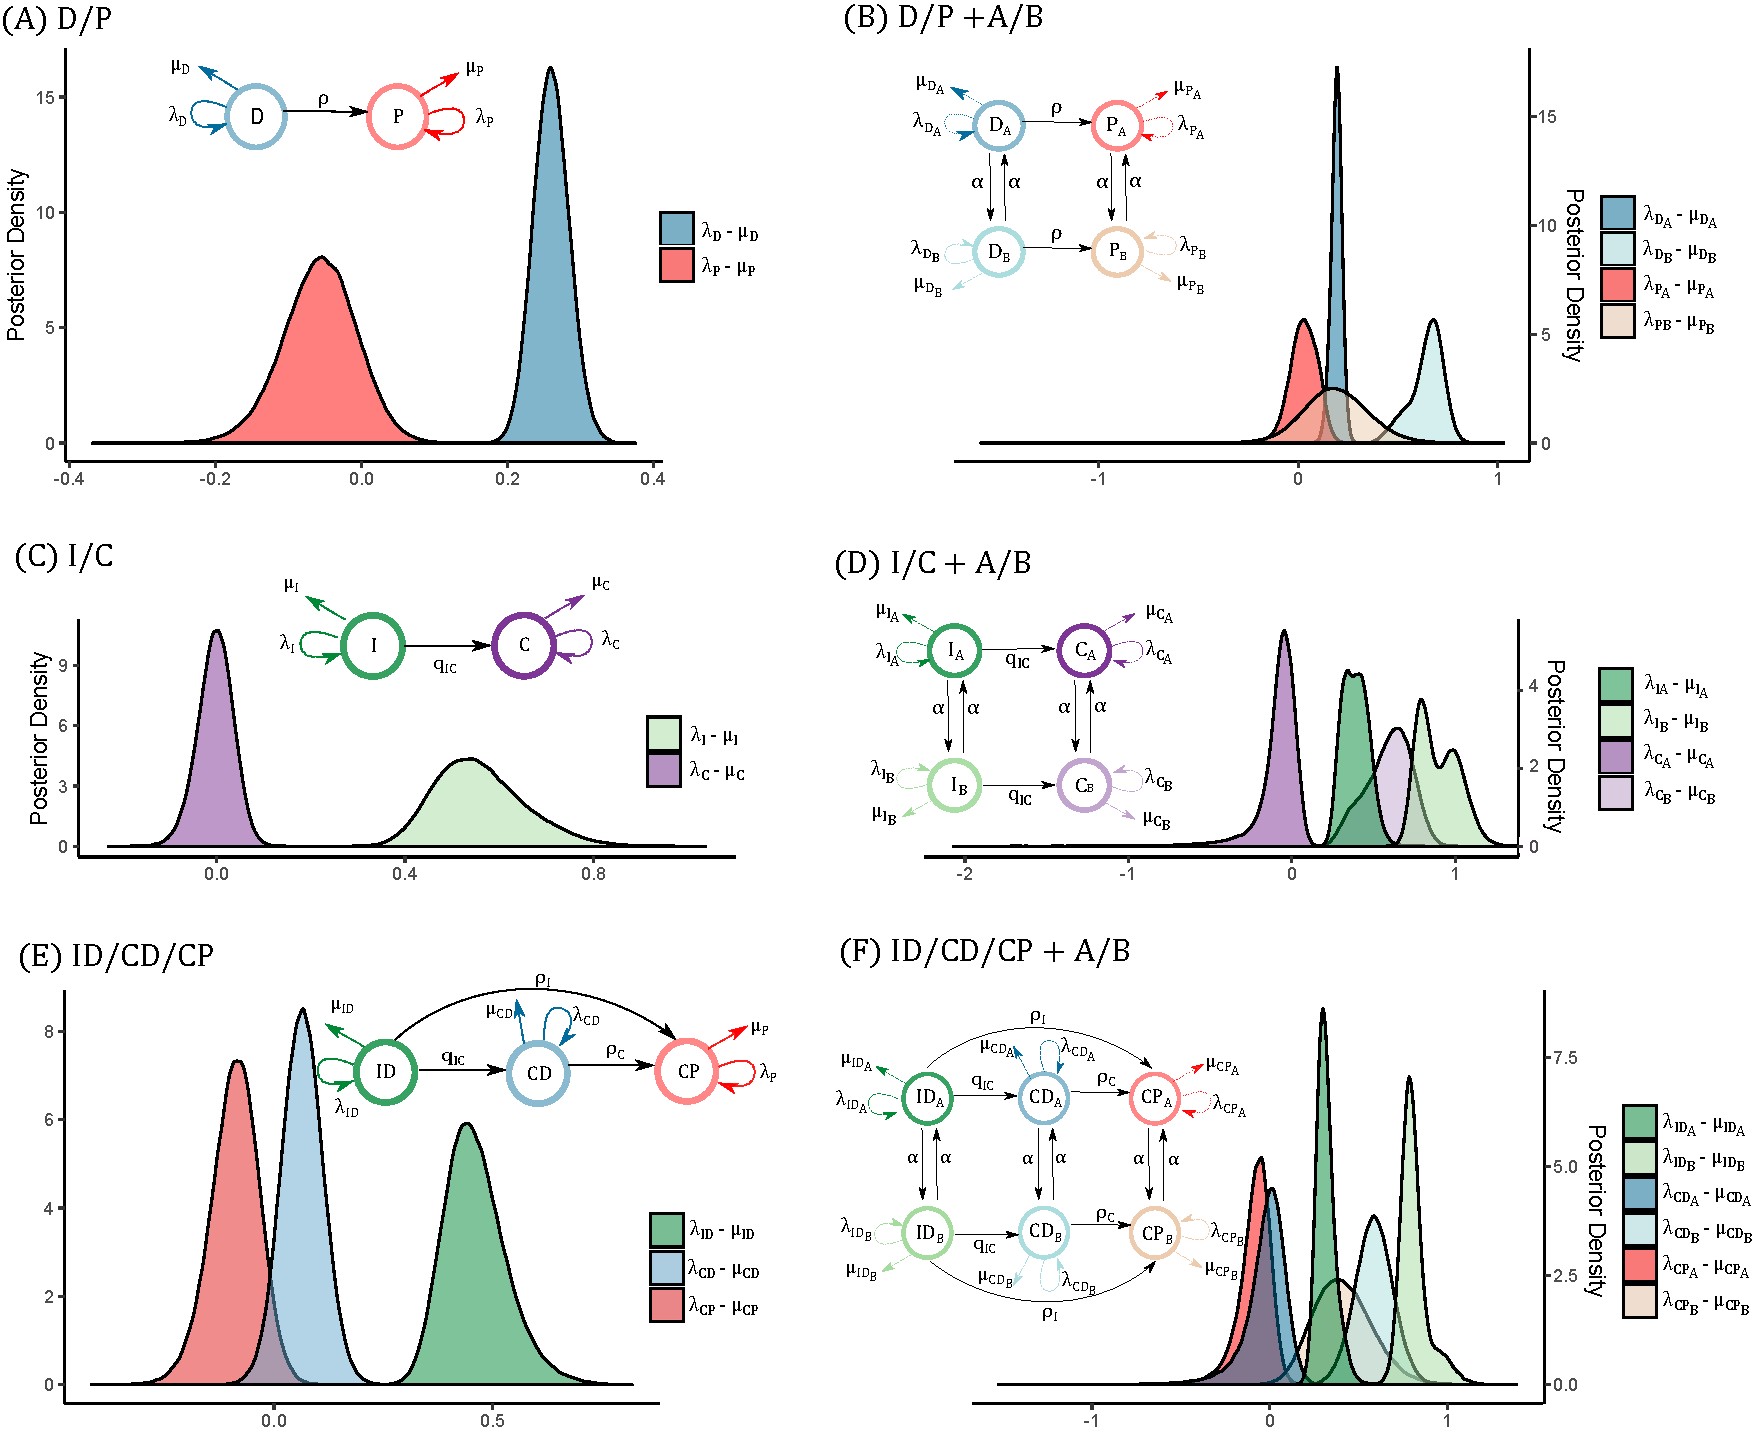
\includegraphics[width=\textwidth]{allnetdivmodelswithoutdelta.pdf} % FIXME: The panel labels should use "+A/B" instead of "-A/B".  Rosana, if you add the .svg file for this figure, I can make small changes like this.
\caption{Net diversification rates for all models.}  
\label{figure:netdivall}
\end{figure}

\begin{figure}
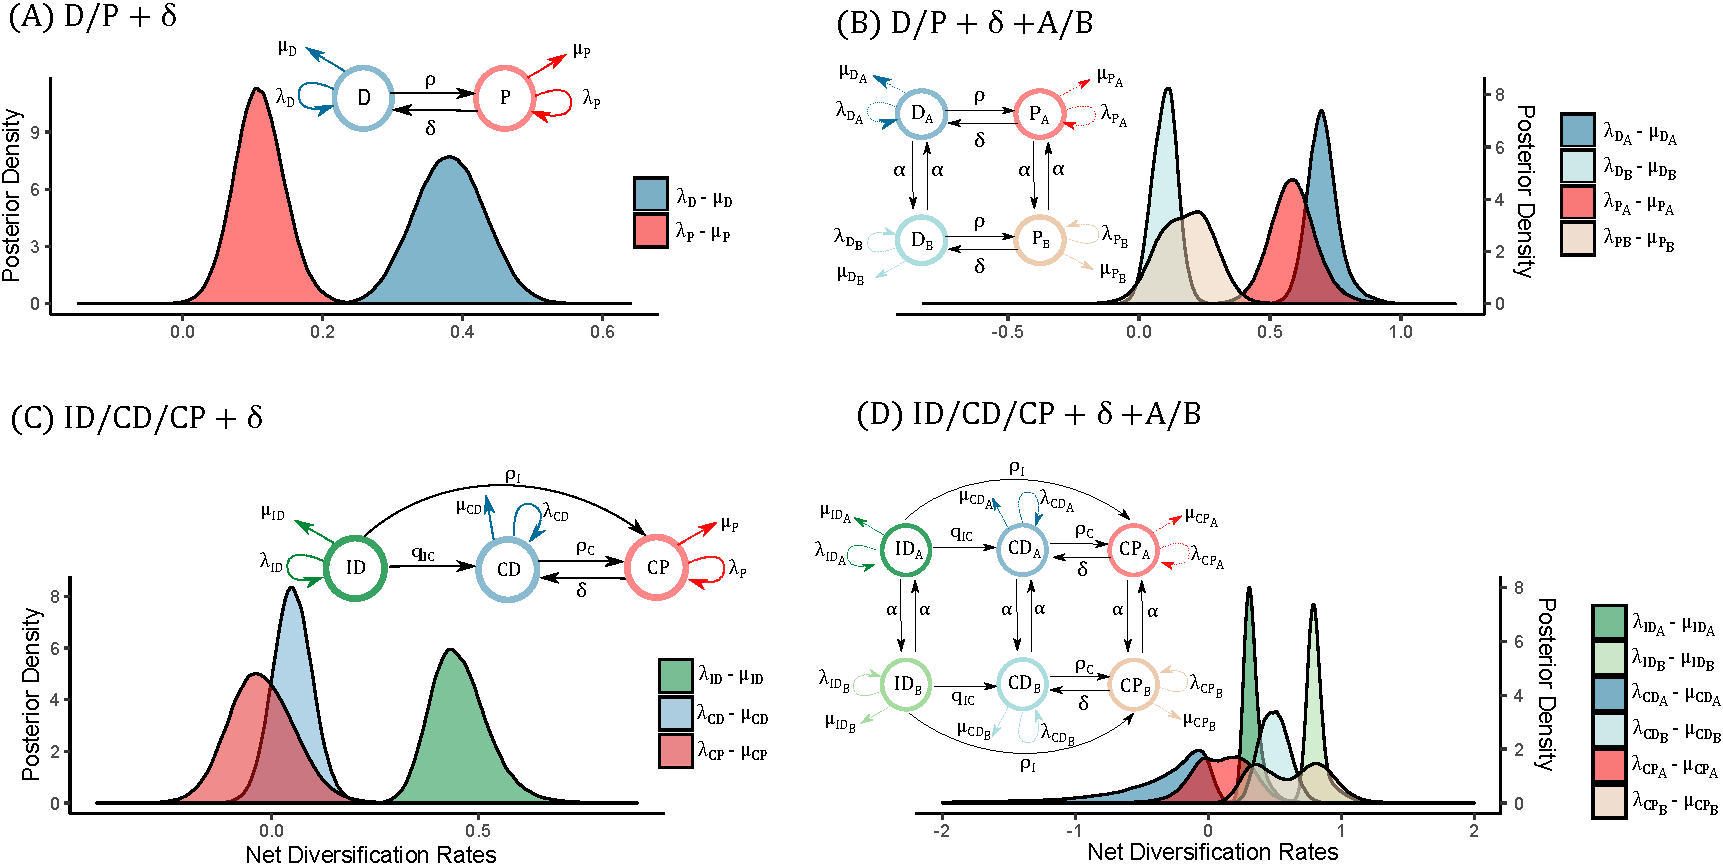
\includegraphics[width=\textwidth]{allnetdivmodelsdiploidization.pdf} % FIXME: same note as above about "+A/B"
\caption{Net diversification rates for all models that include diploidization.}  
\label{figure:netdivnodip}
\end{figure}

% E todo: could make this look a little less klunky
\begin{figure}
    \centering 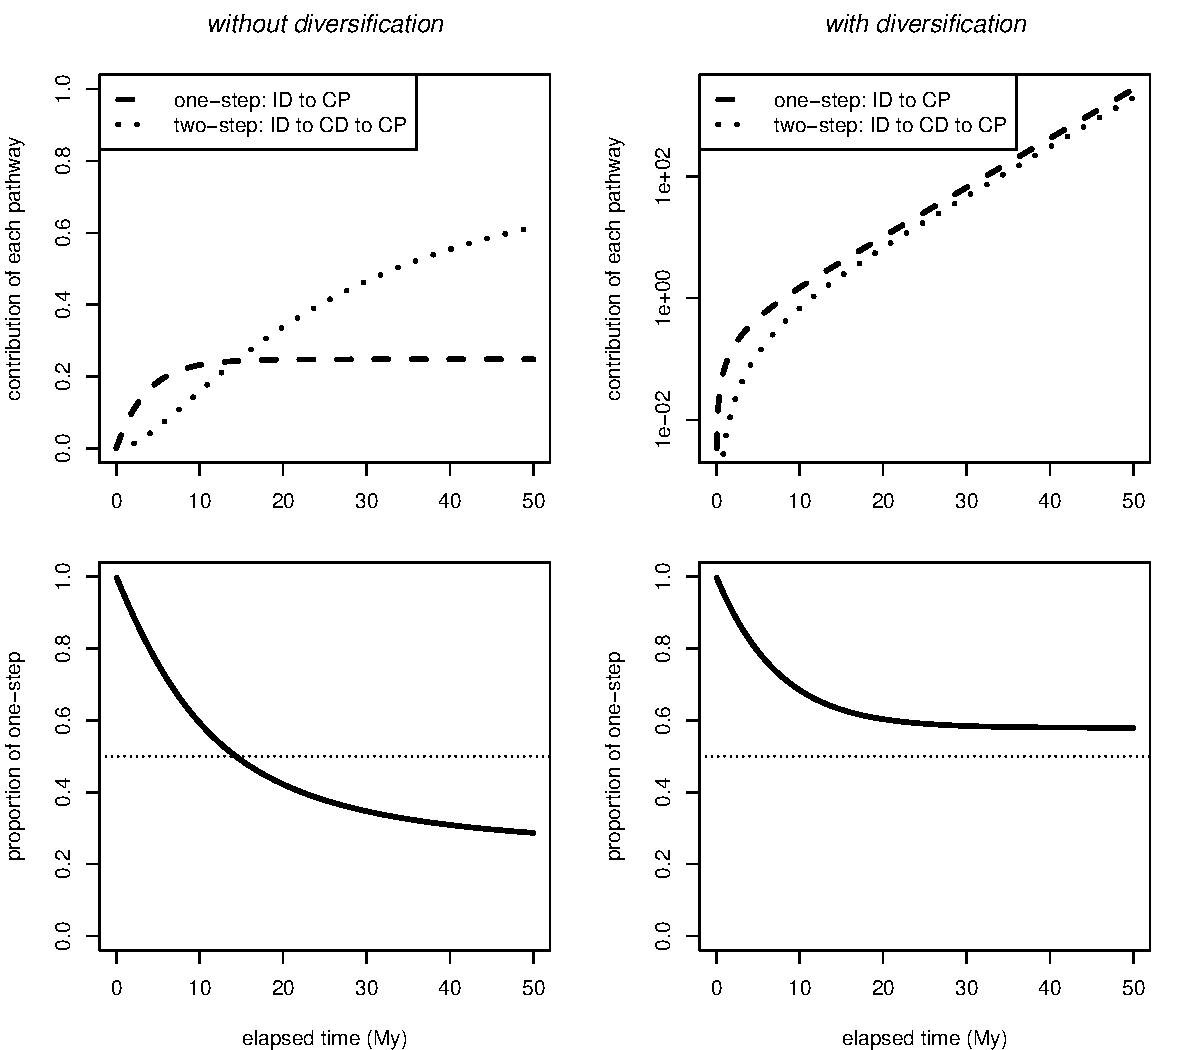
\includegraphics[width=0.9\textwidth]{pathways}
    \caption{
        %B: FIXME: R&E check this re-wording to see if it is to your liking--I think I clarified it a bit, although with length increase.
        %Contributions of the two pathways to polyploidy.
        %When considering only rates of transitions among the states (left), the one-step pathway dominates on short timescales and the two-step on long timescales.
        %When also considering diversification within each state (right), the one-step pathway dominates over any timescale.
        %The lower panels plot the ratio of the two pathway contributions in the upper panels.
        Contributions of the two pathways to polyploidy, the one-step ID$\rightarrow$CP transitions, and the two-step, ID$\rightarrow$CD$\rightarrow$CP transitions.
        Panel (a) shows the contributions when considering only transition rates among the states (ignoring the diversification rate parameters). 
        The one-step pathway dominates on short timescales and the two-step on long timescales.
        Panels (b) shows the contributions when including diversification of lineages in each state. 
        The one-step pathway, in which polyploidy breaks down SI, dominates over any timescale.
        Panels (c) and (d) plot the ratio of the pathway contributions in the upper panels, (a) and (b), respectively.
    }
    
    
    \label{figure:pathways}
\end{figure}

\begin{suppfigure}
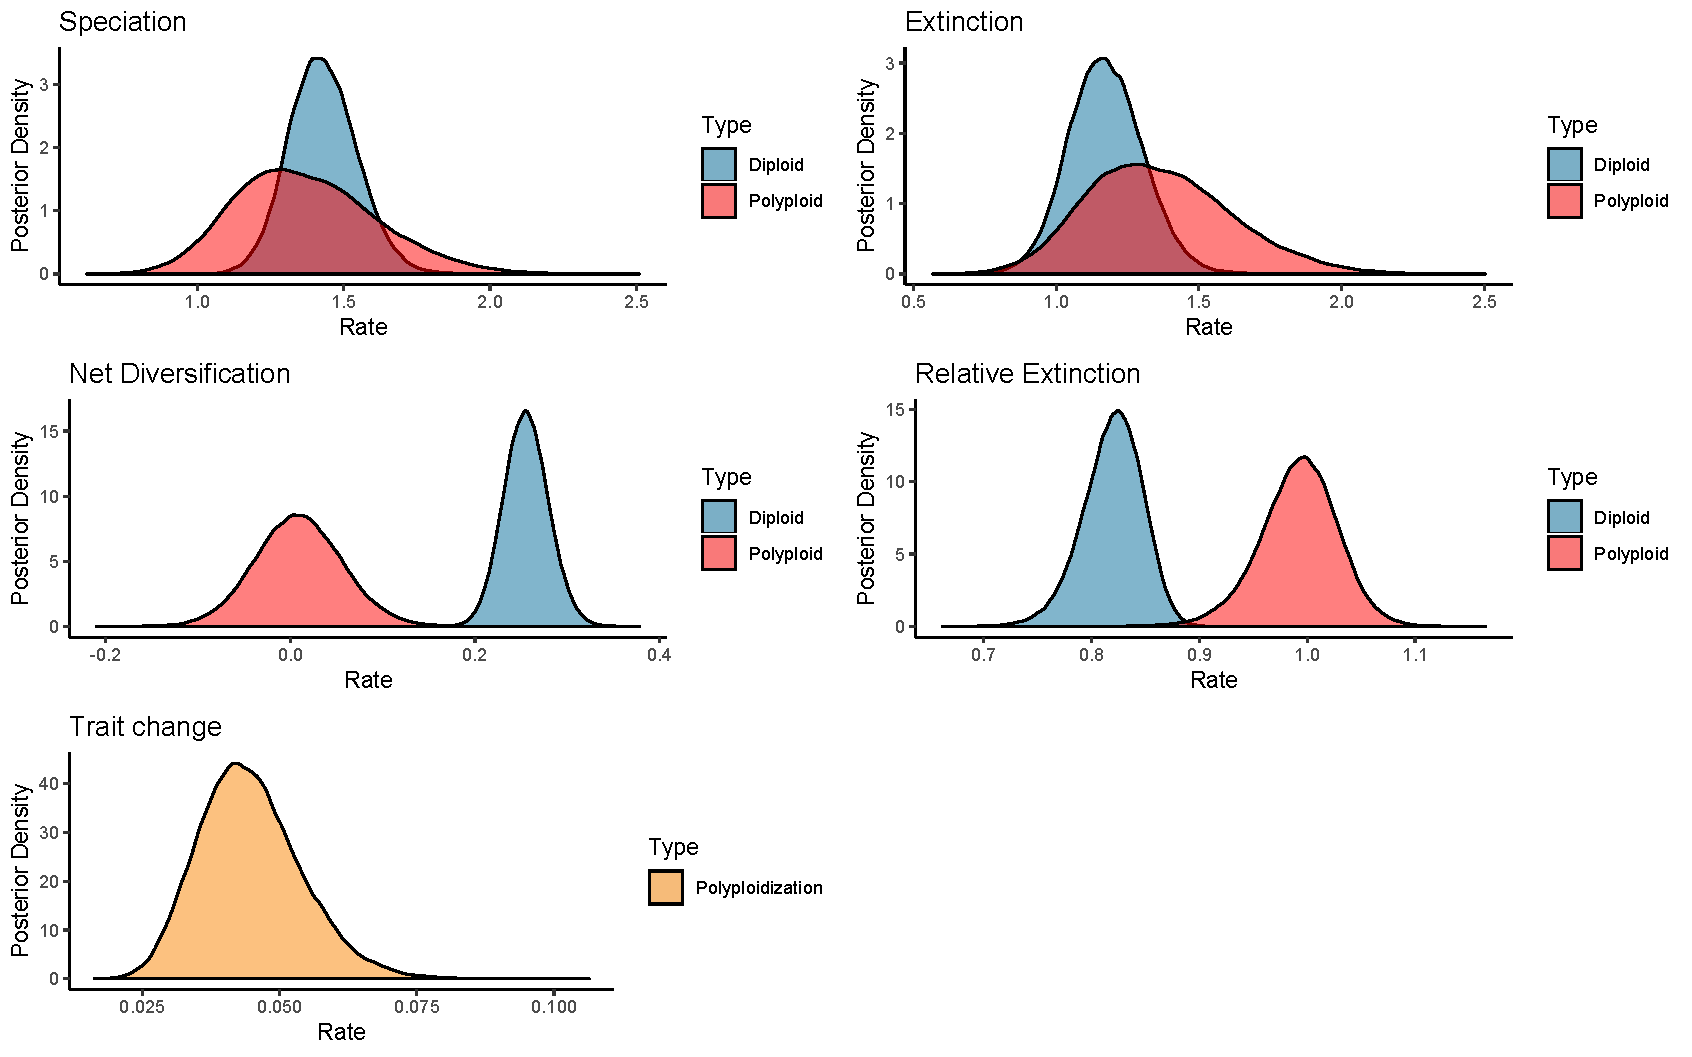
\includegraphics[width=\textwidth]{bisseDPnodipposteriordist.pdf}
\caption{Posterior distribution for each of the parameters in the D/P, polyploidy model} % XXX
\label{suppfigure:DPnodip}
\end{suppfigure}

\begin{suppfigure}
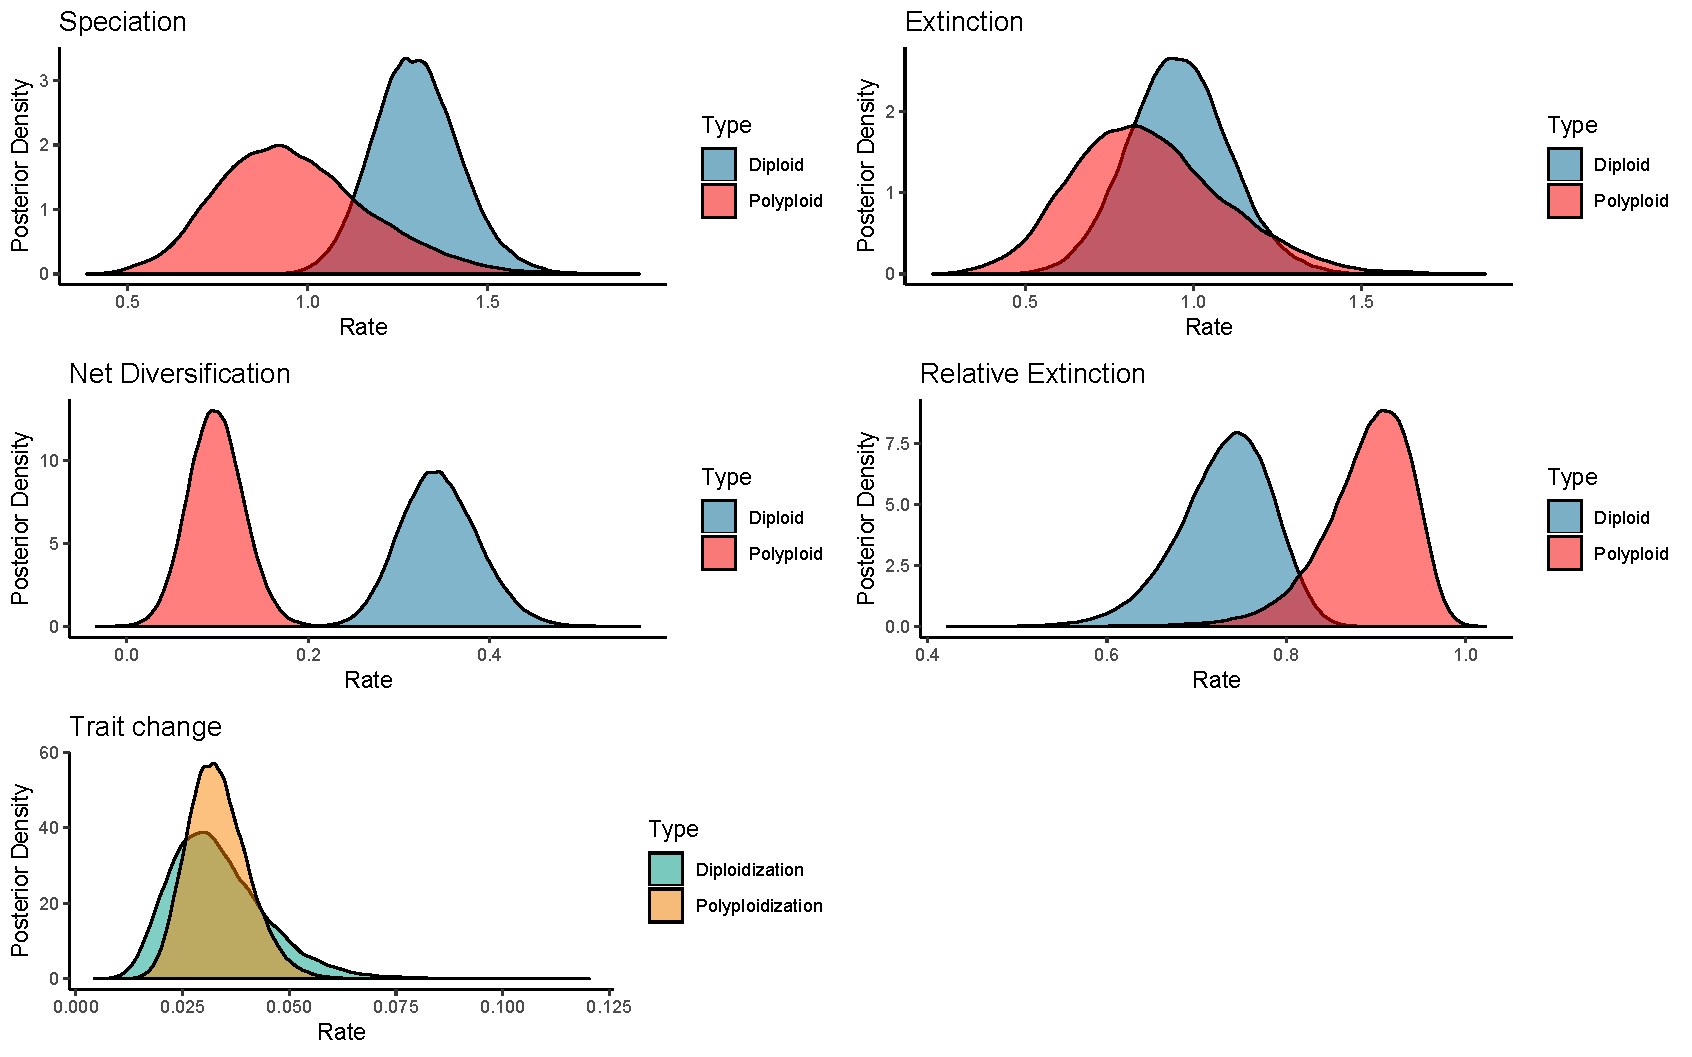
\includegraphics[width=\textwidth]{bisseDPposteriordist.pdf}
\caption{Posterior distribution for each of the parameters in the D/P+ $\delta$,polyploidy model} % XXX
\label{suppfigure:DP}
\end{suppfigure}

\begin{suppfigure}
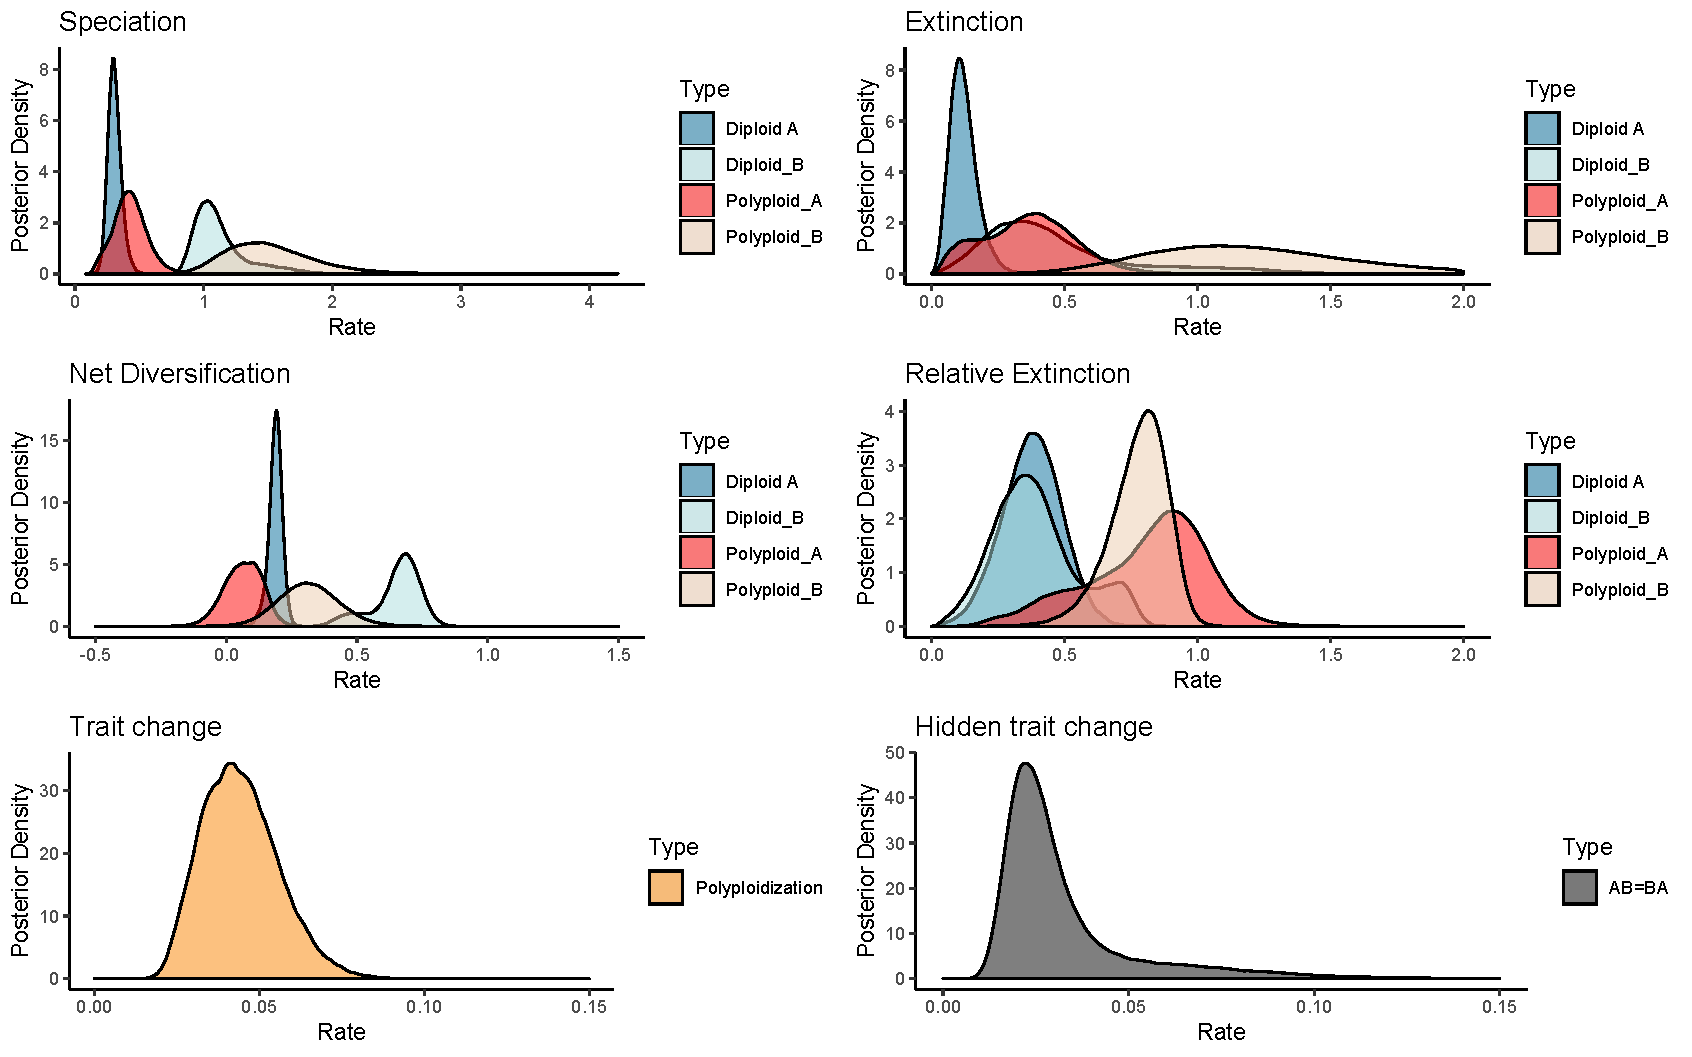
\includegraphics[width=\textwidth]{hisseDPnodipposteriordist.pdf}
\caption{Posterior distribution for each of the parameters in the D/P+A/B, polyploidy model} % XXX
\label{suppfigure:DPnodipAB}
\end{suppfigure}


\begin{suppfigure}
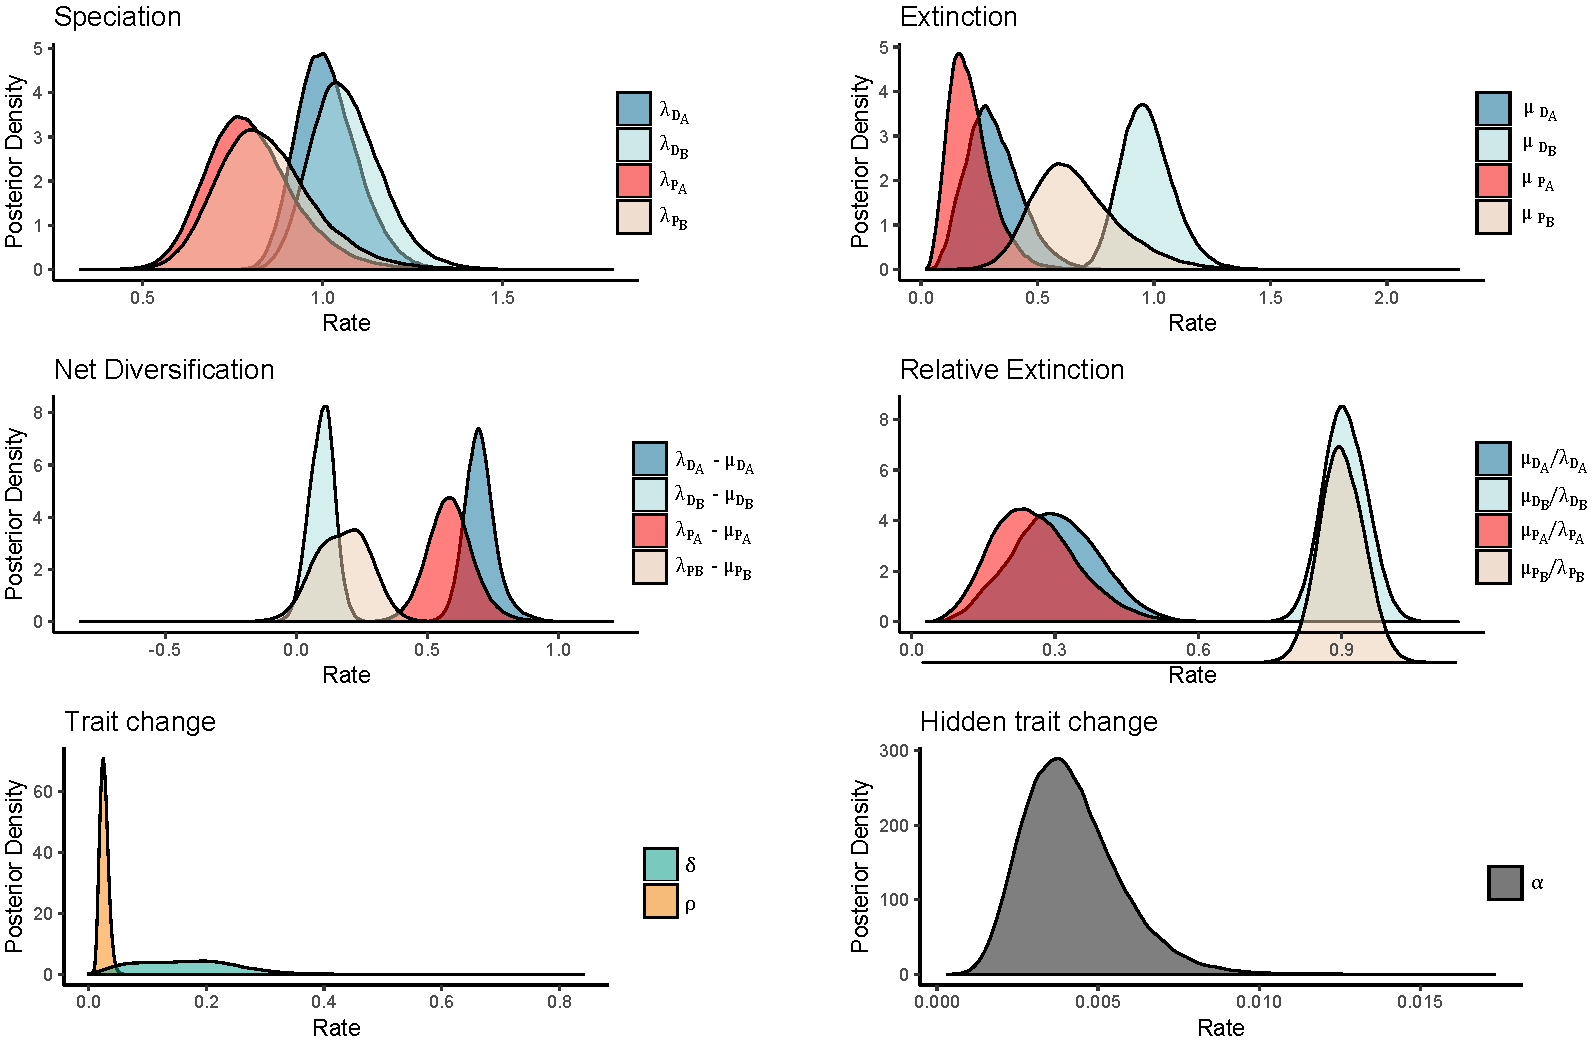
\includegraphics[width=\textwidth]{hisseDPposteriordist.pdf}
\caption{Posterior distribution for each of the parameters in the D/P+$\delta$+A/B, polyploidy model.  The axis is offset in one location so that the two overlapping distributions can be seen.} % XXX
\label{suppfigure:DPAB}
\end{suppfigure}


\begin{suppfigure}
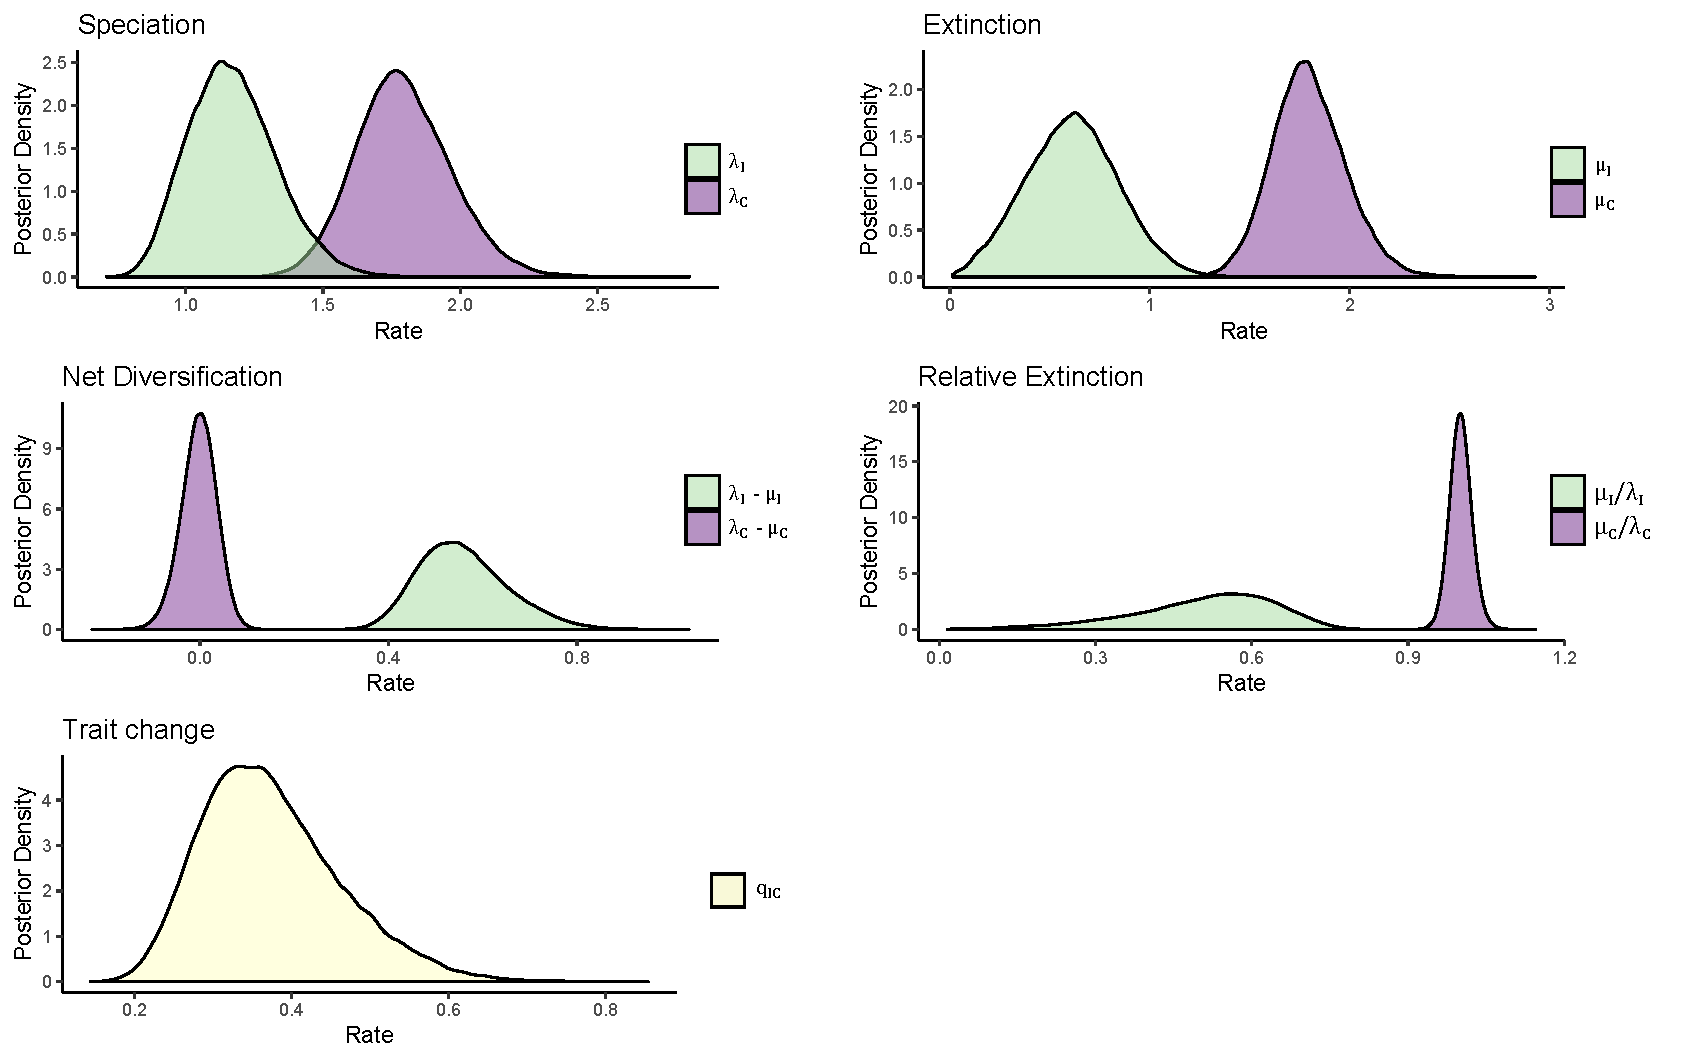
\includegraphics[width=\textwidth]{bisseSIposteriordist.pdf}
\caption{Posterior distribution for each of the parameters in the I/C, breeding system model} % XXX
\label{suppfigure:IC}
\end{suppfigure}

\begin{suppfigure}
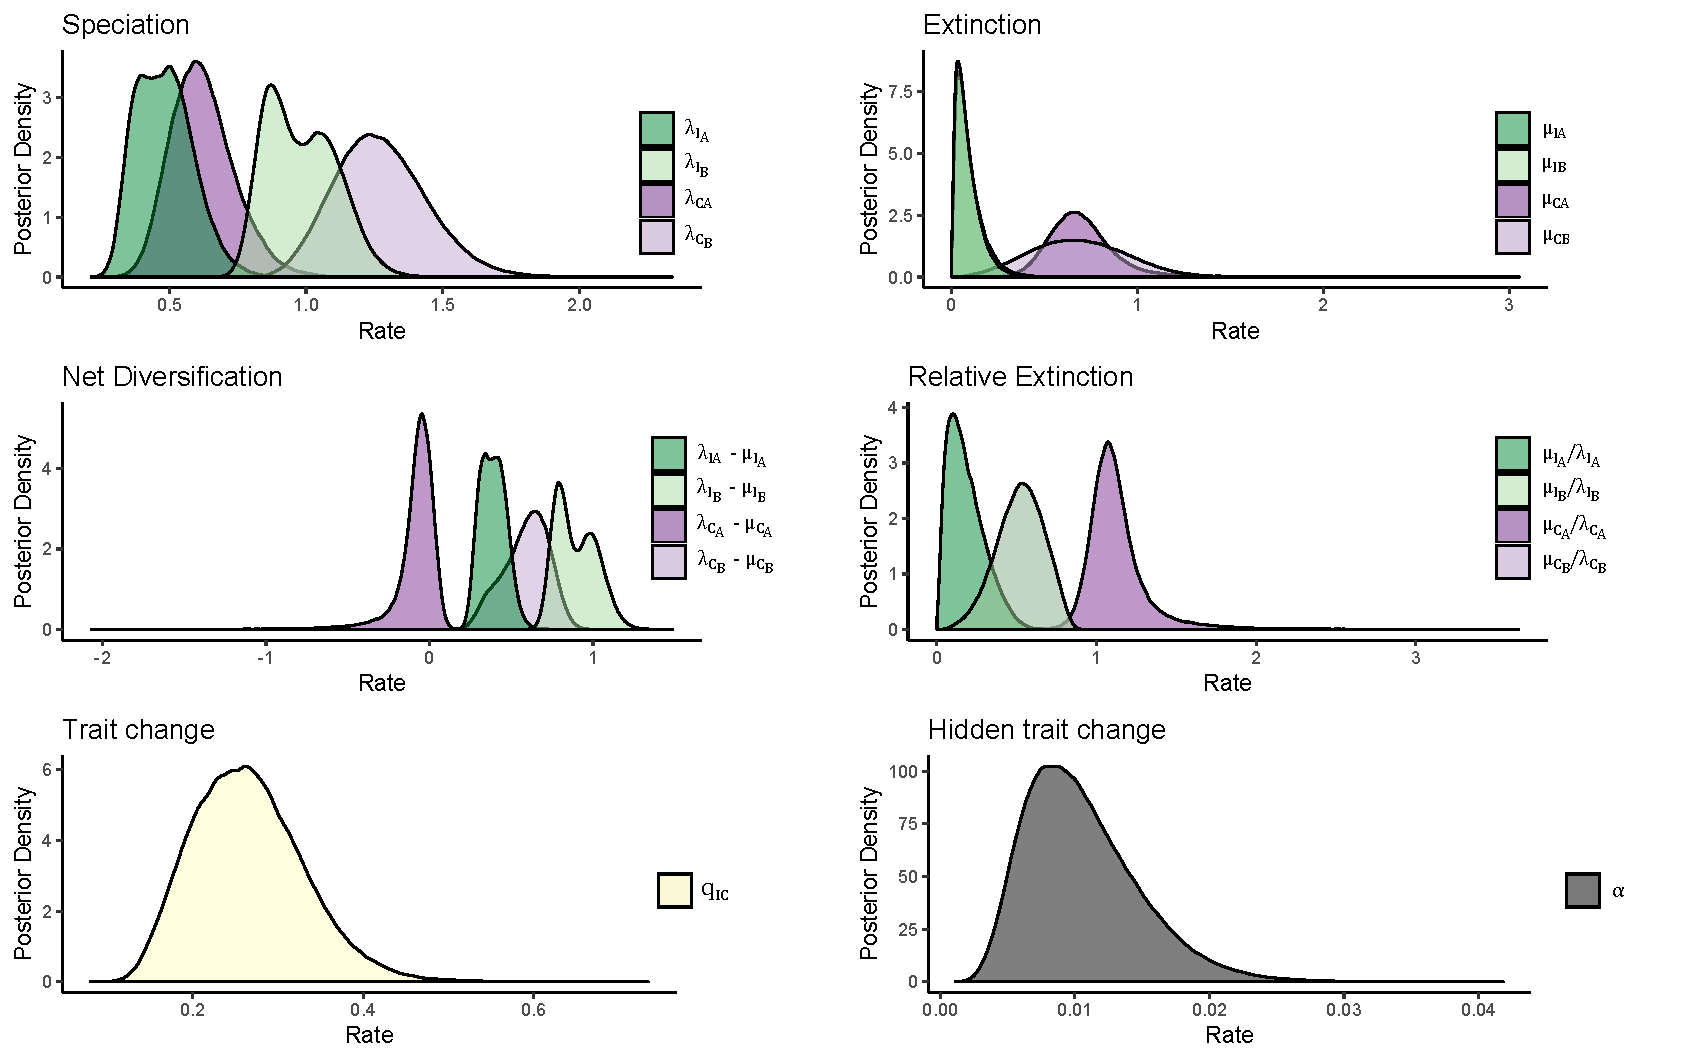
\includegraphics[width=\textwidth]{hisseSInoretposteriordist.pdf}
\caption{Posterior distribution for each of the parameters in the I/C+A/B, breeding system model} % XXX
\label{suppfigure:ICAB}
\end{suppfigure}

\begin{suppfigure}
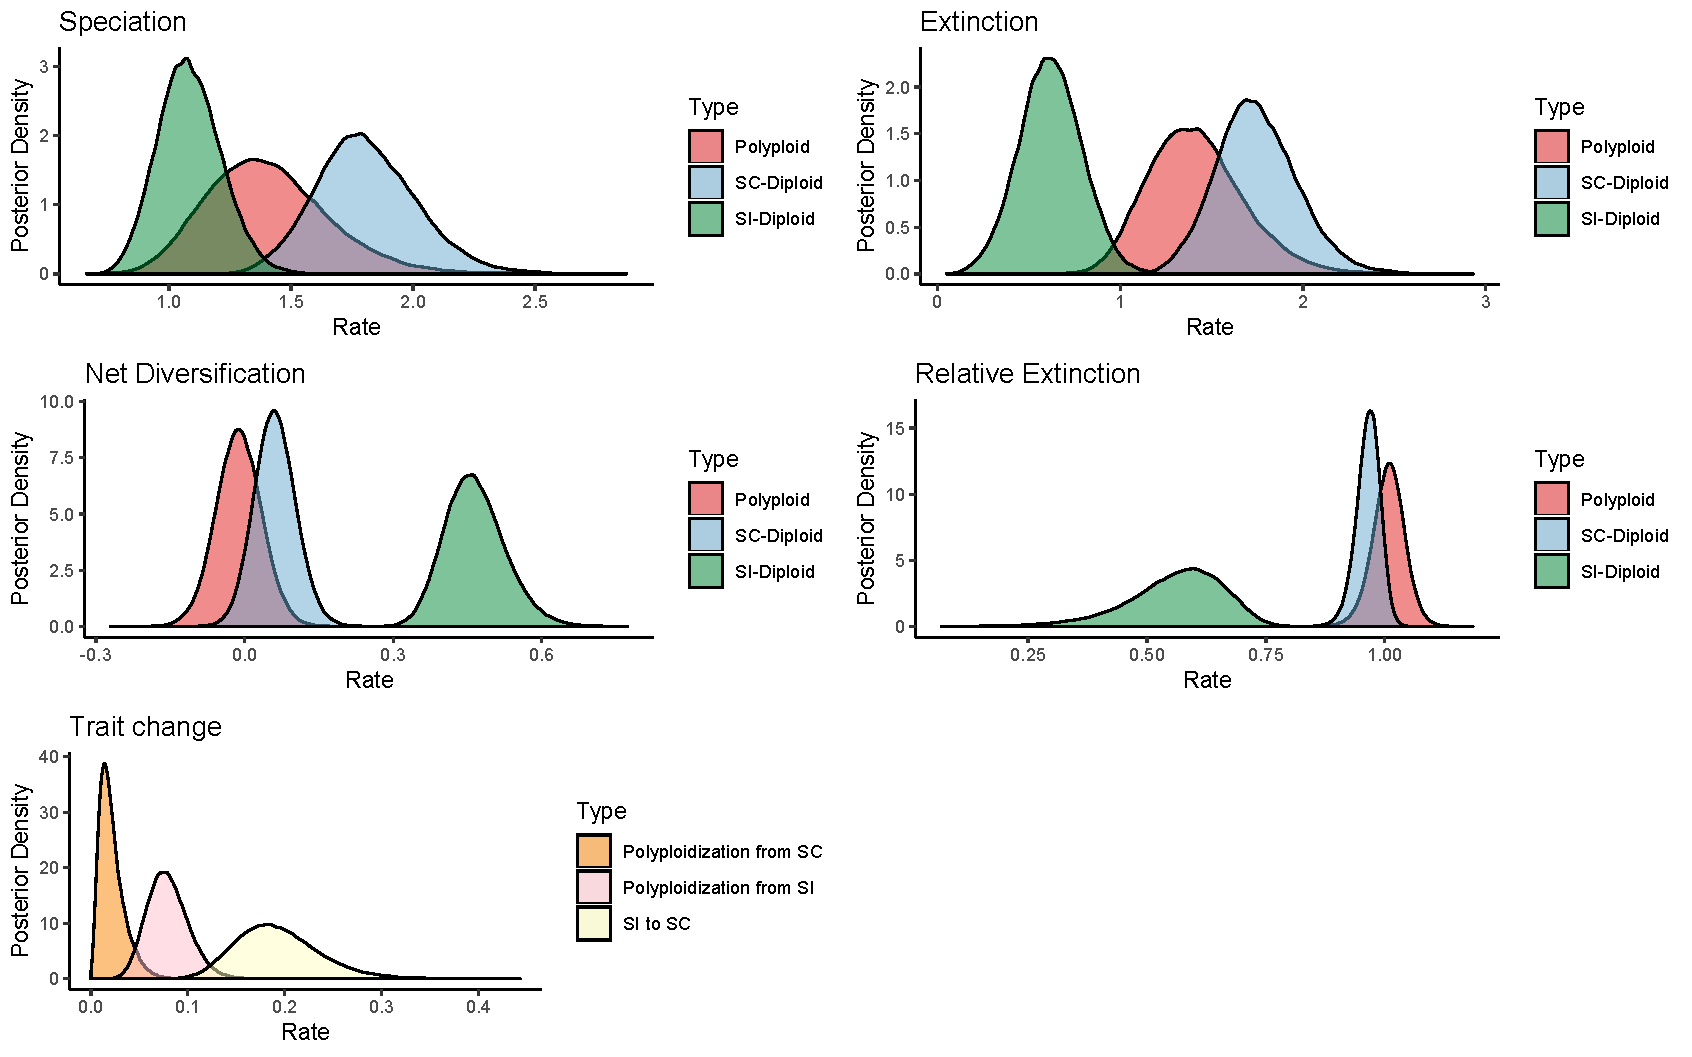
\includegraphics[width=\textwidth]{musseDPSInodipposteriordist.pdf}
\caption{Posterior distribution for each of the parameters in the ID/CD/CP, polyploidy and breeding system model} % XXX
\label{suppfigure:IDCDCPnodip}
\end{suppfigure}

\begin{suppfigure}
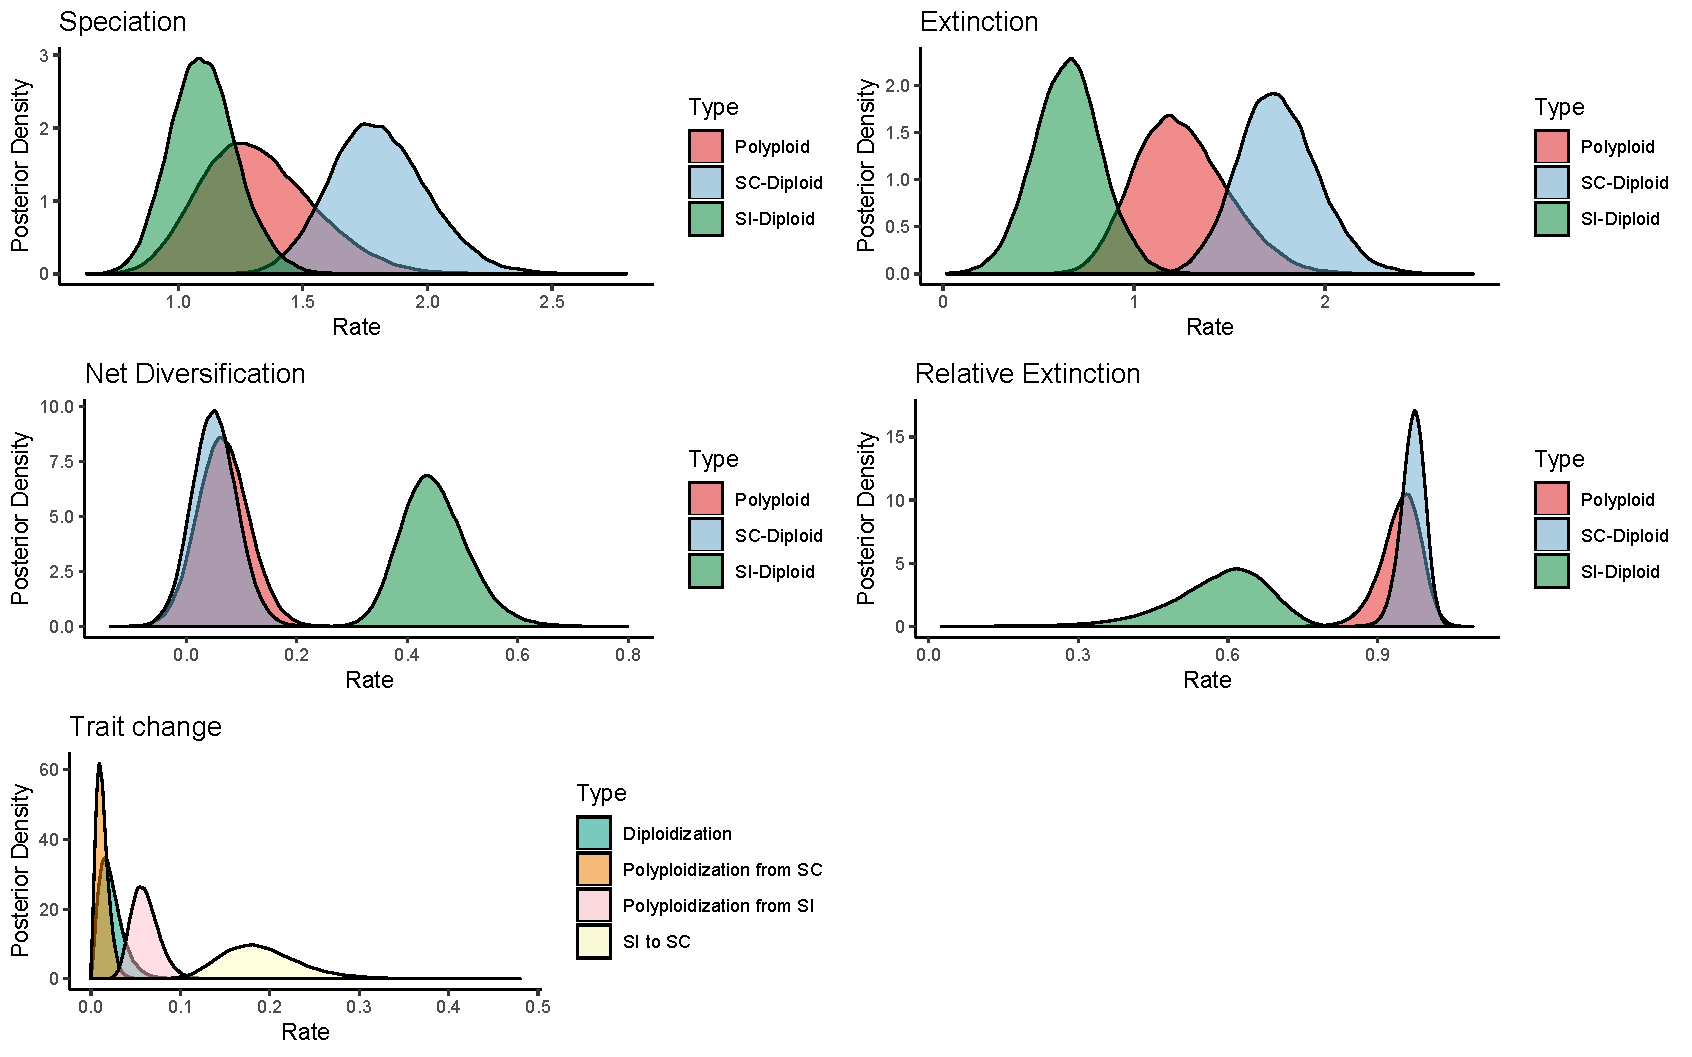
\includegraphics[width=\textwidth]{musseDPSIposteriordist.pdf}
\caption{Posterior distribution for each of the parameters in the ID/CD/CP+$\delta$, polyploidy and breeding system model} % XXX
\label{suppfigure:IDCDCP}
\end{suppfigure}

\begin{suppfigure}
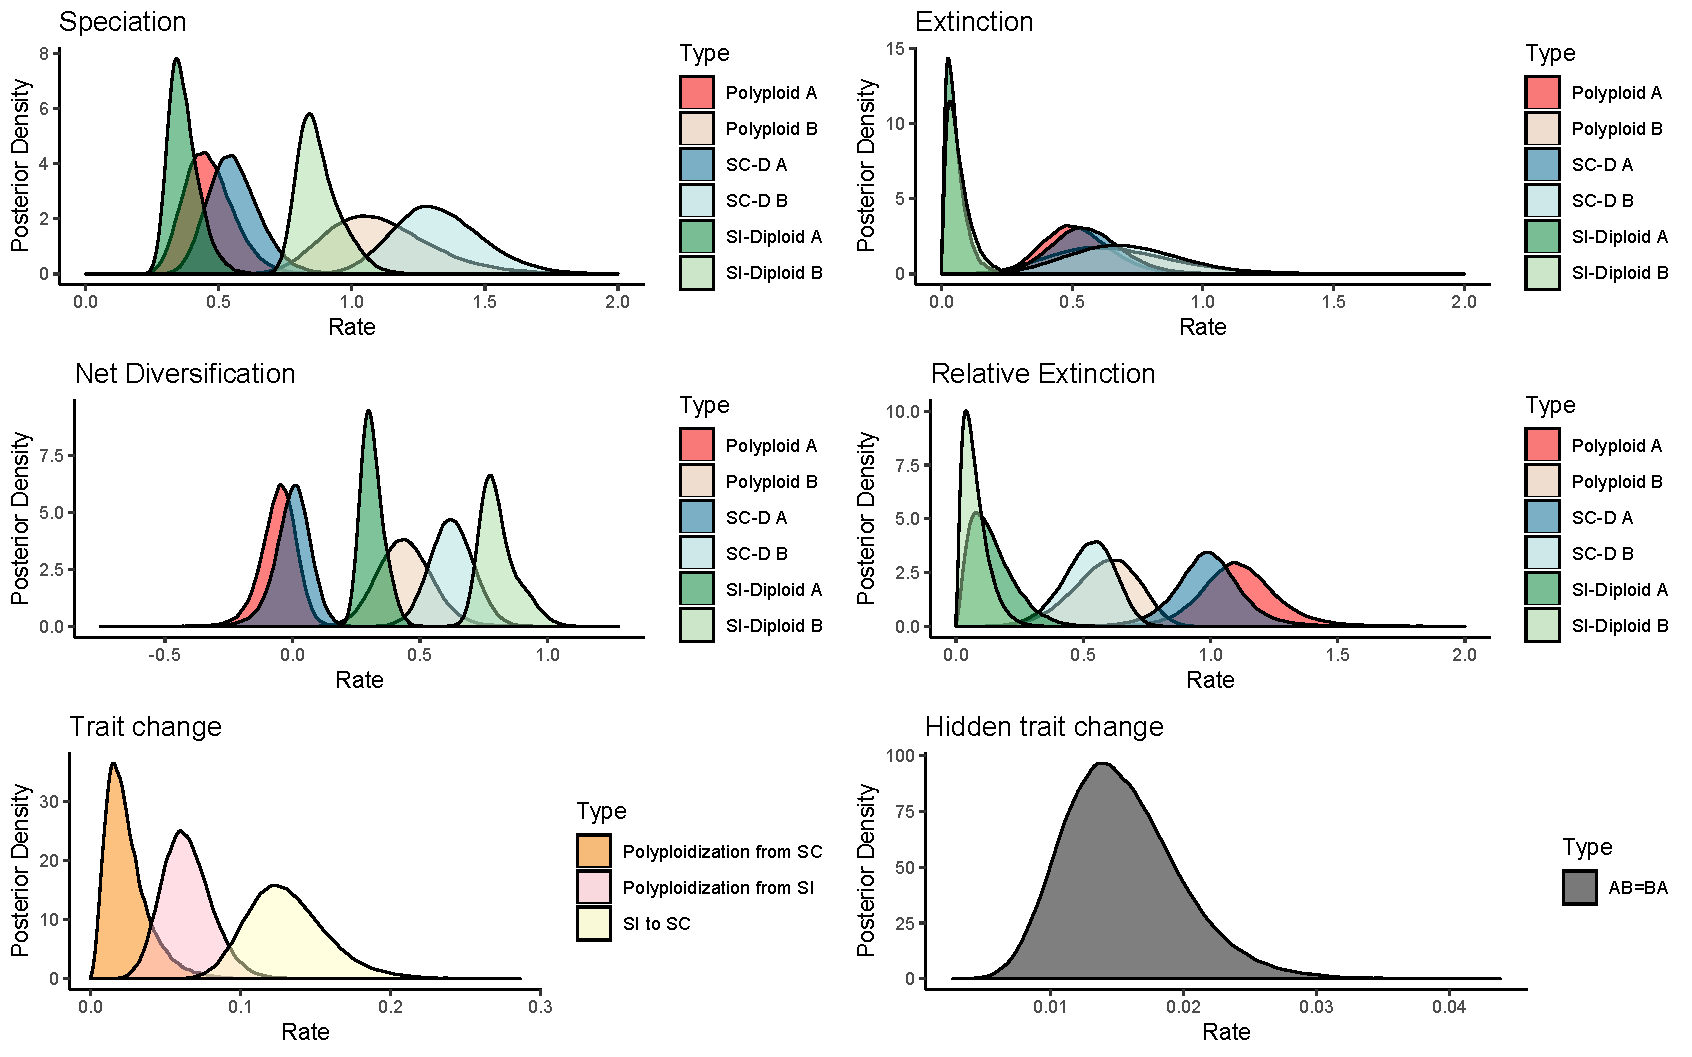
\includegraphics[width=\textwidth]{muhisseDPSInodipposteriordist.pdf}
\caption{Posterior distribution for each of the parameters in the ID/CD/CP+A/B polyploidy and breeding system model} % XXX
\label{suppfigure:IDCDCPnodipAB}
\end{suppfigure}

\begin{suppfigure}
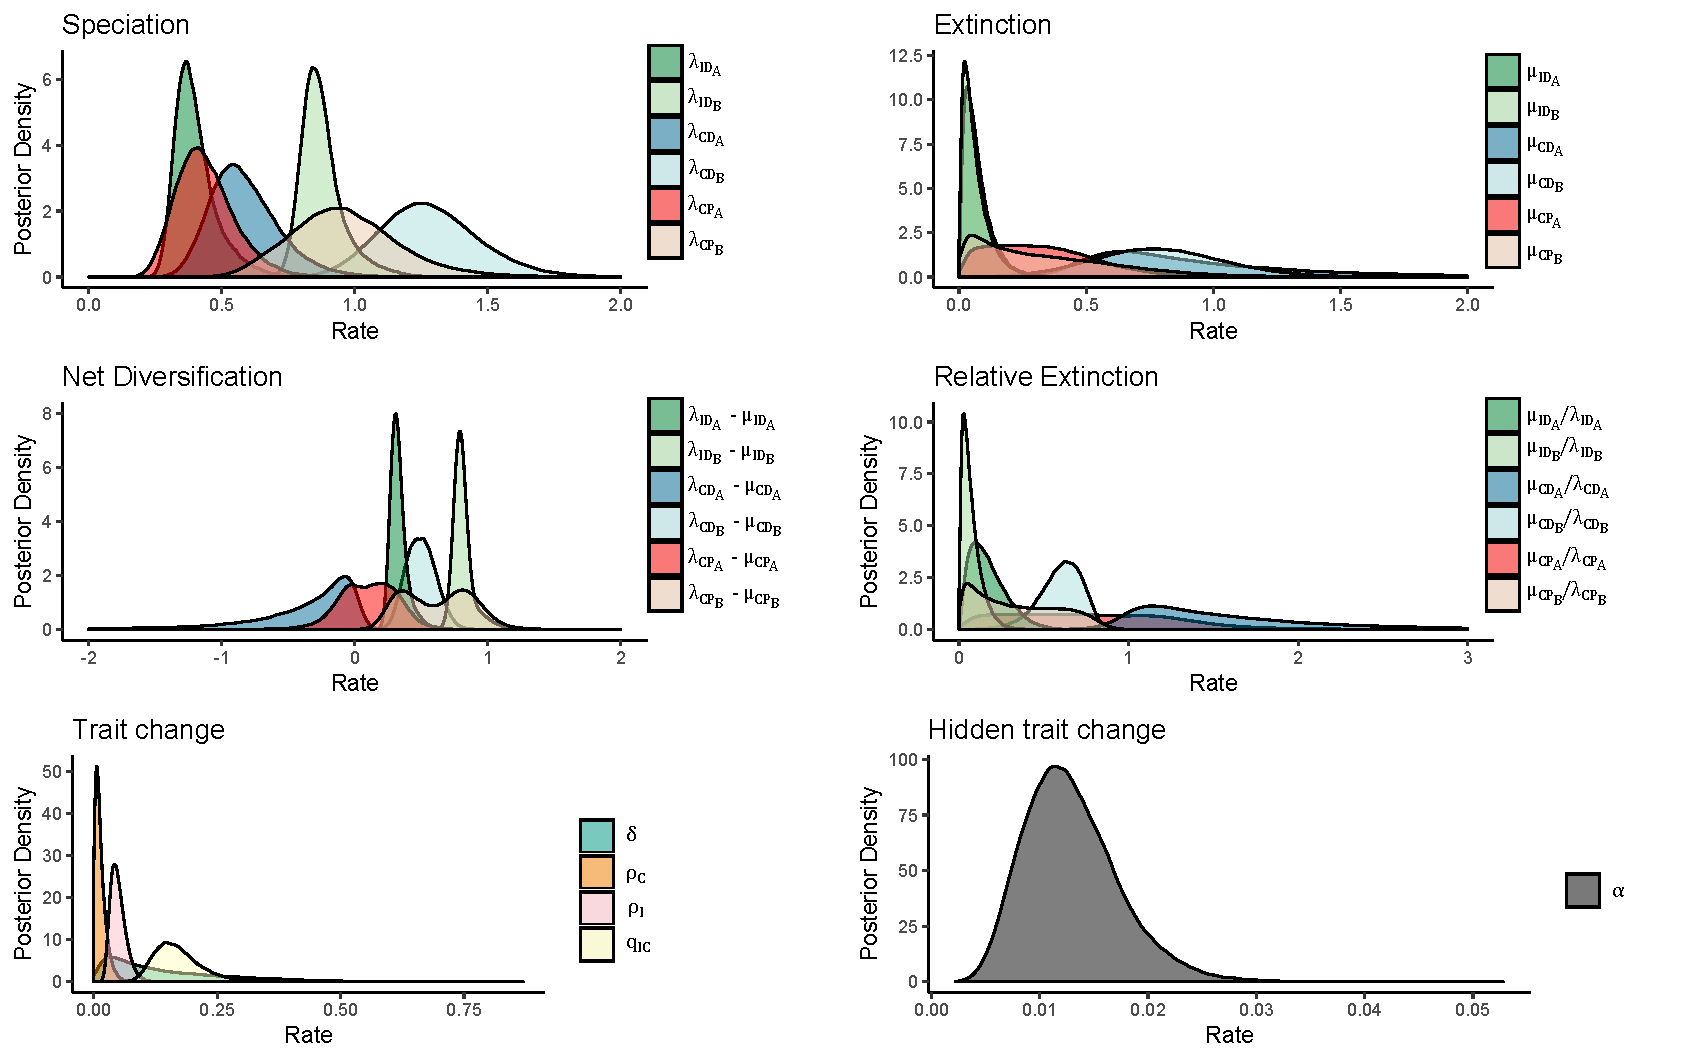
\includegraphics[width=\textwidth]{muhisseDPSIposteriordist.pdf}
\caption{Posterior distribution for each of the parameters in the ID/CD/CP+$\delta$+A/B, polyploidy and breeding system model} % XXX
\label{suppfigure:IDCDCPAB}
\end{suppfigure}


